%%%%%%%%%%%%%%%%%%%%%%%%%%%%%%%%%%%%%%%%%%%%%%%%%%%%%%%%%%%%%%%%%%%%%%%%%%%%%%%%%%%%%%%%%%%%%%%%%%%%%%%

\documentclass[prb,aps,12pt,superscriptaddress,floatfix]{revtex4-2} 
\usepackage{graphicx}
\usepackage{color} 
\usepackage{amsmath}
\usepackage{amssymb} 
\usepackage{natmove}
\usepackage{natbib}
\usepackage{hyperref} 
\usepackage{bm}

%%%%%%%%%%%%%%%%%%%%%%%%%%%%%%%%%%%%%%%%%%%%%%%%%%%%%%%%%%%%%%%%%%%%%%%%%%%%%%%%%%%%%%%%%%%%%%%%%%%%%%%

\begin{document}

\title{\huge On the Origin of Shrimpoluminescence }

\author{\large Tyler C. Sterling}
\email{ty.sterling@colorado.edu}
%\affiliation{Department of Physics, University of Colorado at Boulder, Boulder, Colorado 80309, USA}

\date{\today}

%\begin{abstract}
%    abstract
%\end{abstract}

\maketitle

%\listoffigures
%\listoftables
%\tableofcontents

%%%%%%%%%%%%%%%%%%%%%%%%%%%%%%%%%%%%%%%%%%%%%%%%%%%%%%%%%%%%%%%%%%%%%%%%%%%%%%%%%%%%%%%%%%%%%%%%%%%%%%%

\begin{figure}
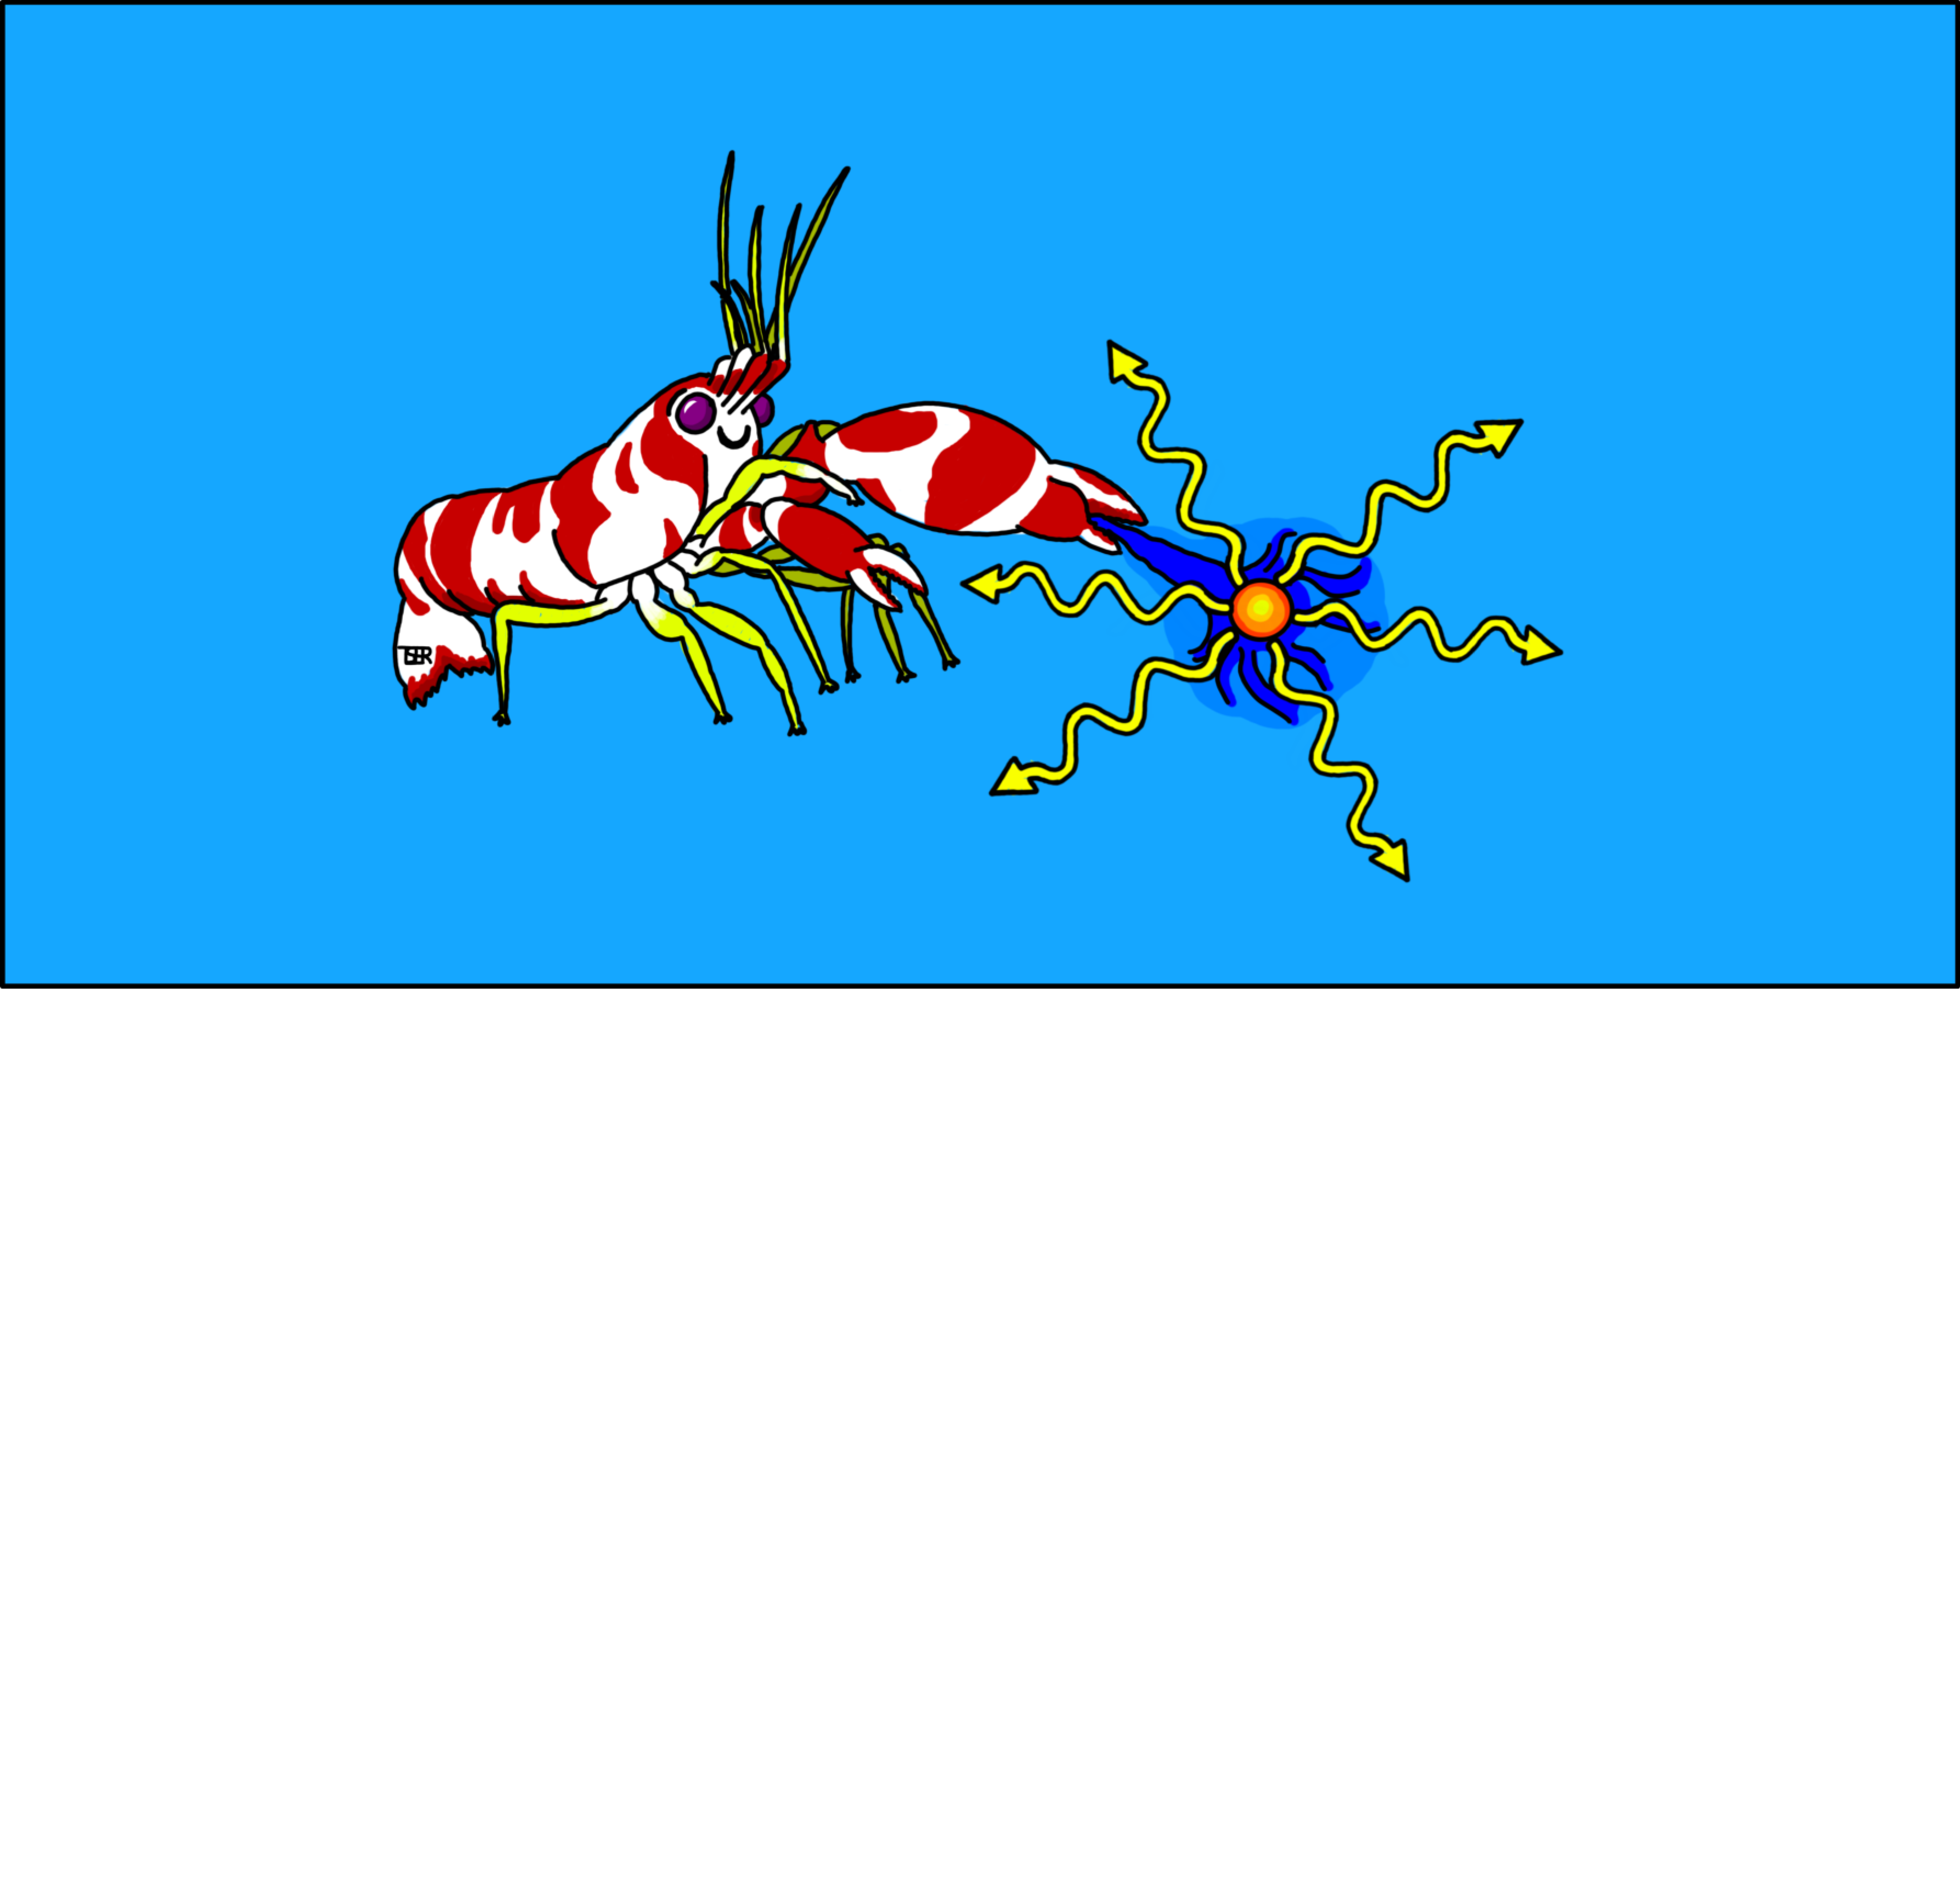
\includegraphics[width=1\linewidth]{figs/shrimpy2.pdf}
%    \caption{}
\label{fig:shrimpy}
\end{figure}

 
\newpage

\section{Details...}
Pistol shrimp, like the red-banded pistol shrimp shown on the cover, are capabale of generating a jet of water with high enough velocity that a cavitation bubble forms behind it. When the bubble collpases, enough energy is released to produce a shock-wave that can kill the shrimp's prey \cite{}. If the shrimp's prey had very sensitive eyes (and also weren't dead) they might notice a flash of light produced through an effect referred to as ``shrimpoluminescence" in the case of the pistol shrimp \cite{}, but more generally known as \emph{sonoluminescence} \cite{}.

Sonolumiscence is more precisely defined as ... \cite{} and occurs in a number of scenarios where cavitation occurs ... \cite{}. Yet the physical origin of light production in sonolumiscence is not understood. To-date, there are two \emph{prevailing} theories: (i) it is a thermally induced phenomena \cite{} and (ii) it is an electrical effect \cite{}. I will review both of these ideas, describing both the theory and experiments. The thermal school of thought has focused a lot of effort on measuring the temperature of the bubble when light is emmited and estimates are in the \emph{thousands} of Kelvin (the surface of the Sun is ... K! \cite{}) so some time will be spent discussing this.

On the other hand, I can't ignore an ``alternative" theory which is actually what led me to this topic: a phenomenological theory based on quantum electrodynamics. This subject will get us out of the main scope of the paper (and into an area that I probably can't answer questions about) but I plan to spend a small amount of time on this too because, well... it sounds interesting!

\section{About me}

My undergraduate degree is in manufacturing where I worked with industrial robots on manufacturing process optimization. I also completed a masters degree in materials science at CU before transferring into the physics PhD program. In the materials science program, I worked in the aerospace department using molecular dynamics to study (lattice) thermal conductivity in thermoelectrics. I work for Dmitry Reznik so my research is still focused on lattice-dynamics, but my methods are based on computational electronic-structure theory(i.e DFT). We usually look at fancy materials like cuprates or magnets, but we also study energy materials like thermoelectrics and hybrid perovskites. The point is, none of this is even closely related to shrimpoluminscence. I plan to have fun writing this paper and I hope you will have fun reading it! 



%%%%%%%%%%%%%%%%%%%%%%%%%%%%%%%%%%%%%%%%%%%%%%%%%%%%%%%%%%%%%%%%%%%%%%%%%%%%%%%%%%%%%%%%%%%%%%%%%%%%%%%

\bibliography{ref}

\end{document}
